\documentclass[../main.tex]{subfiles}
\begin{document}
\setchapterstyle{kao}
\setchapterpreamble[u]{\margintoc}
%INIZIO LEZIONE 10/06
\chapter[A closer look to Lorentz and Poincaré group]{A closer look to Lorentz and Poincaré groups\footnotemark[0]}
\labch{LPgroups}
\section{Foreword}
From the mathematical viewpoint, this is a corollary of what we already did! $\textrm{SO}(p,q)$ is the generalized orthogonal group, with $p,q\in\mathbb{N}$ and $p+q=n$. The Lorentz group is just the name we give to $p=1$ and $q=3$\index{Lorentz group}
\[
\mathcal{L}:=\textrm{SO}(1,3)\quad  \textrm{Lorentz group}
\]
and, as we are going to see, there is a \textbf{double covering}:
\[
\Phi:\text{SL}(2,\mathbb{C})\overset{\textrm{Lie hom}}{\twoheadrightarrow}\mathcal{L} \quad \ker\Phi=\{+\mathbb{1},-\mathbb{1}\}
\]
As $\textrm{SL}(2,\mathbb{C})$ is simply connected, it is the universal covering group of the Lorentz group. Moreover, we already know $\textrm{irrep}(\mathfrak{sl}(2,\mathbb{C}))$: they are classified by a single \textbf{half-integer} number\marginnote{In the physicists' notation, mathematicians use instead integer numbers.}  $s\in\frac{1}{2}\mathbb{N}$: the "\textbf{spin}" of the representation. Since SL$(2,\mathbb{C})$ is also \textbf{semi-simple}, by Bargmann's theorem [\vrefthm{bargmann}] every \textbf{projective unitary representation} is equivalent to a (true) \textbf{unitary representation}. 

From the Physics viewpoint: things have different "names" suggesting different "interpretations". Hence, we are going to use the physicists' convention.
\section{Lie algebra of the Poincaré group}
Since the Poincaré group $\pazocal{P}$ is $\pazocal{P}=\pazocal{L}\rtimes\mathbb{R}^4$, we have that:
\[
\dim\pazocal{P}=\dim\mathcal{L}+\dim\mathbb{R}^4=10
\]
We introduce the generators of the space-time translations $(P^0\equiv H,P^1,P^2,P^3)$, which are called the components of the momentum operator\index{Momentum operator}, then we introduce the Lorentz group generators $J^{\mu\nu}=-J^{\nu\mu}$. We take a look at the commutation relations:\marginnote{$H$ is not precisely the Hamiltonian operator, it is a tangent vector to the Poincaré group whose representation in the Hilbert space will be the Hamiltonian operator, once we hve a unitary representation of the operators in the Hilbert space.

$\eta$ is the \textbf{Minkowski metric}:
\[
\eta=\left(\begin{array}{cccc}
    -1 & 0 & 0 & 0 \\
    0 & +1 & 0 & 0 \\
    0 & 0 & +1 & 0 \\
    0 & 0 & 0 & +1
\end{array}\right)
\]}
\[
\left\{
\begin{aligned}
&i[J^{\mu\nu},J^{\rho\sigma}]=\eta^{\nu\rho}J^{\mu\sigma}-\eta^{\mu\rho}J^{\nu\sigma}-\eta^{\sigma\mu}J^{\rho\nu}+\eta^{\sigma\nu}J^{\rho\mu}\\
&i[P^\mu,J^{\rho\sigma}]=\eta^{\mu\rho}P^\sigma-\eta^{\mu\sigma}P^\rho\\
&[P^\mu,P^\nu]=0
\end{aligned}
\right.
\]
\subsection{Physical reinterpretation}
The physical interpretation of the generators is the following, where we have separated the $J^{\mu\nu}$ into two groups:
\[
\begin{cases}
P^0\equiv H &\textrm{Hamiltonian}\\
\mathbb{P}=(P^1,P^2,P^3) &\textrm{Linear momentum}\\
\mathbb{J}=(J^{23},J^{31},J^{12}) &\textrm{Angular momentum}\\
\mathbb{K}=(J^{10},J^{20},J^{30}) &\textrm{Boosts' generators}
\end{cases}
\]
Be careful because the components of the linear momentum and the components of the angular momentum all commute with the Hamiltonian, so they are conserved in time and we can use them to label quantum space. Vice versa the boosts' generators do not commute with the Hamiltonian, so they are not conserved and they are not a good label, nevertheless they are physically very relevant. Looking at commutation relations now give us:
\[
\begin{cases}
[J_i,J_j]=i\varepsilon_{ijk}J_k &\xrightarrow[]{}\text{angular momentum commutation rule, $\textrm{SO}(3)\cong\textrm{SU}(2)$}\\
[J_i,K_j]=i\varepsilon_{ijk}K_k&\xrightarrow[]{}\mathbb{K}=(K_1,K_2,K_3) \text{ is a SO(3)-vector}\\
[K_i,K_j]={\color{red}-}i\varepsilon_{ijk}J_k&\xrightarrow[]{}\text{\textbf{Thomas precession} (the - comes from the metric)}\\
[J_i,P_j]=i\varepsilon_{ijk}P_k&\xrightarrow[]{}\mathbb{P}\text{ is a SO(3)-vector}\\
[K_i,P_j]=iH\delta_{ij}\\
[K_i,H]=iP_i\\
[J_i,H]=[P_i,H]=0
\end{cases}
\]
The minus in the Thomas precession comes from the fact that the metric has a $-1$, therefore from the fact that we are talking about the Lorentz group and not about the orthogonal group in 4-dimensions.
%42:00
\section{Topology of the Lorentz group}
We will do exactly the trick of the two brothers [\refch{Two-brothers}]:\\ $\textrm{SL}(2,\mathbb{C})\twoheadrightarrow\mathcal{L}$.
\begin{itemize}
    \item We identify space-time points $(x^0,x^1,x^2,x^3)\in\mathbb{M}$ with $2\times2$ complex matrices:
    \[
    X=\sum_{\mu=0}^3x^\mu\sigma_\mu=\left(\begin{array}{cc}
    x_0+x_3 & x_1-ix_2 \\
    x_1+ix_2 & x_0-x_3
\end{array}\right)
    \]
    where $\sigma_0=\mathbb{1}$ and $(\sigma_1,\sigma_2,\sigma_3)$ are the \href{https://en.wikipedia.org/wiki/Pauli_matrices}{Pauli matrices}. So, in a sense, we are identifying 
    \[
    {\color{red}\mathbb{M}\xrightarrow[]{\cong}\text{Her}(\mathbb{C}^2)_{\mathbb{R}}=i\mathfrak{u}(2)}
    \]
    \item Now we let SL(2,$\mathbb{C}$) act on Her$(\mathbb{C}^2)\cong\mathbb{M}$ via:
    \[
    {\color{red}\Phi_{\Lambda}(X)=\Lambda X \Lambda^* \quad \Big|\Big| \quad \star}\marginnote{With $\Lambda^*$ we denote the complex conjugate. Here it is more convenient to use the conjugation rather than the inverse, it is possible to use $\Lambda^{-1}$ in the case that it is unitary.}
    \]
    Notice that Her$(\mathbb{C}^2)$ is preserved by the action of $\Phi_\Lambda$:
    \[
    \Phi_\Lambda(X)^\ast=(\Lambda X \Lambda^*)^*=\Lambda X^*\Lambda^*\underset{\mathclap{\tikz \node {$\uparrow$} node [below=1ex] {\footnotesize $X$ is hermitian};}}{=}\Lambda X \Lambda^*=\Phi_\Lambda(X) \quad \checkmark
    \]
    \item The Minkowski metric $\|x\|^2_h=-x_0^2+x_1^2+x_2^2+x_3^2$ is represented in Her$(\mathbb{C}^2)$ by the determinant, up to a minus:
    \[
    {\color{red}\|x\|^2_h=-\det X}
    \]
    After the action of $\Phi_\Lambda$ with $\Lambda\in\textrm{SL}(2,\mathbb{C})$:
    \[
    \det(\Phi_\Lambda(X))=\det(\Lambda X \Lambda^*)\underset{\mathclap{\tikz \node {$\uparrow$} node [below=1ex] {\footnotesize Binet's formula };}}=\det(\Lambda)\det (X)\det(\Lambda^*)=|\det(\Lambda)|^2\det (X)\underset{\mathclap{\tikz \node {$\uparrow$} node [below=1ex] {\footnotesize $\Lambda\in\textrm{SL}$};}}{}=\det X \quad \checkmark
    \]
    Up to an identification, we have {\color{red}$\Phi_{\Lambda}\in\textrm{SO}(1,3)$}.
    \item We have a \textbf{Lie group homomorphism}:
    \begin{align*}
    \text{SL}(2,\mathbb{C})&\xrightarrow[]{}\text{SO}(1,3)\equiv\mathcal{L}\\
    \Lambda&\mapsto\Phi_\Lambda
    \end{align*}
    We might notice that
    \begin{itemize}
        \item $\Phi_\Lambda$ preserves the Minkowski metric;\\
        \item $\Phi_{\Lambda_1\Lambda_2}=\Phi_{\Lambda_1}\circ\Phi_{\Lambda_2}$
    \end{itemize}
    \item One checks that $\Phi$ is \underline{\textbf{surjective}} and its kernel is $\ker\Phi=\{+\mathbb{1},-\mathbb{1}\}$.
    %53:00
\end{itemize}
%1:05:00
\underline{\textbf{Summary:}} we constructed a \textbf{2-fold} covering.
\begin{figure}[h!]
    \centering
    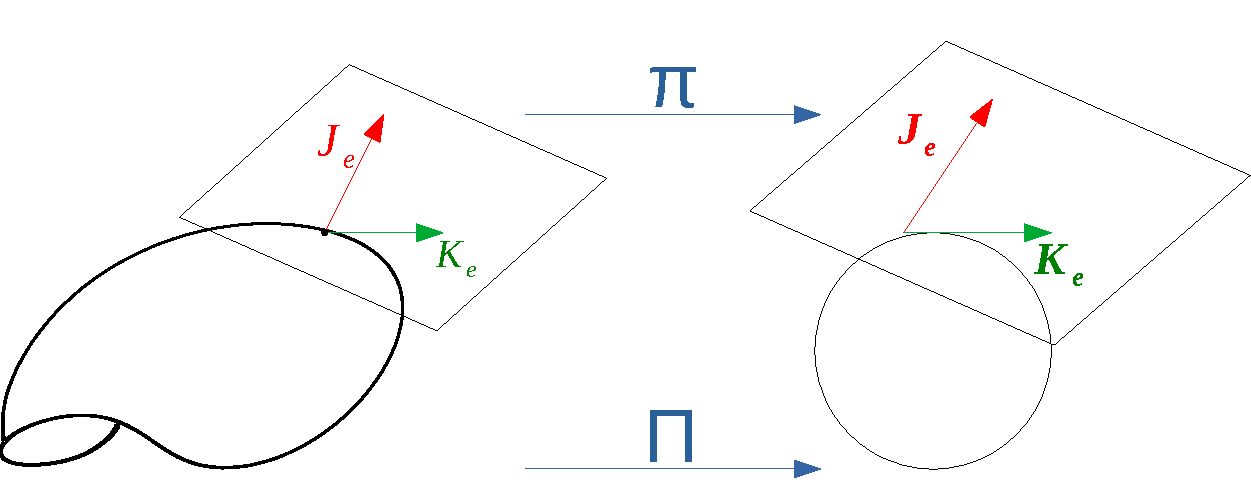
\includegraphics{images/2_fold_covering.pdf}
    \caption{$\Pi$ sends $\mathcal{L}$ to GL(V).}
    \labfig{2_fold_covering}
\end{figure}\\
By using the \textbf{polar decomposition} [\refch{too-pol-dec}], every $\Lambda\in\textrm{SL}(2,\mathbb{C})$ can be written as
\[
\Lambda=Ue^X \quad (X^*=X,U^*U=\mathbb{1})
\]
with the \textbf{constraint} that:
\[
1=\det(\Lambda)\underset{\mathclap{\tikz \node {$\uparrow$} node [below=1ex] {\footnotesize Binet's formula };}}=\det(U)\det (e^X)\underset{\mathclap{\tikz \node {$\uparrow$} node [below=1ex] {\footnotesize Magic formula };}}=\det(U)e^{\tr(X)}\overset{!}{=}1 \xleftrightarrow[]{}\begin{cases}
\det U=1\\
\tr X=0
\end{cases}
\]
This means that there is a direct link between $\Lambda$ and $(U,X)$:
\[
\Lambda\xleftrightarrow[]{}(U,X)\in\text{SU}(2)\times\mathbb{R}^3
\]
\underline{\textbf{Conclusion:}} topologically (not as a group!), we observe that\marginnote{$\approx$ means that it is \textit{topologically identified} or \textit{homeomorphic}, if we want to use the technical word.} 
\[
\textrm{SL}(2,\mathbb{C})\approx\textrm{SU}(2)\times\mathbb{R}^3\approx S^3\times\mathbb{R}^3
\]
Therefore, $\textrm{SL}(2,\mathbb{C})$ is \textbf{simply connected}. Taking now the quotient by $\ker\Phi=\left\{\mathbb{1},-\mathbb{1}\right\}\cong\mathbb{Z}_2$:
\[
{\color{red}\mathcal{L}_0\cong\text{SL}(2,\mathbb{C})/\mathbb{Z}_2\approx\text{SO}(3)\times\mathbb{R}^3}
\]
\begin{corollary}
The Lorentz group is \textbf{not simply connected}!
\end{corollary}
\begin{corollary}
As SL$(2,\mathbb{C})$ is \textbf{simply connected}, every irrep$(\mathfrak{sl}(2,\mathbb{C}))$ induces an irrep of SL$(2,\mathbb{C})$ which satisfies:
\[
\underset{\mathclap{\tikz \node {$\uparrow$} node [below=1ex] {\footnotesize \parbox{1.5cm}{algebra representation}};}}\pi(x)=\dv{t}\underset{\mathclap{\tikz \node {$\uparrow$} node [below=1ex] {\footnotesize \parbox{1.5cm}{group representation}};}}\Pi(e^{tx})\Bigr|_{\substack{t=0}} \quad \forall x\in\mathfrak{sl}(2,\mathbb{C})
\]
\end{corollary}
\begin{corollary}
As SL$(2,\mathbb{C})$ is \textbf{simply connected} and \textbf{semi-simple}, every \textbf{projective unitary representation} is equivalent (up to a "regauging" phase $\Tilde{U}_g=\eta(g)U(g)$) to a (true) \textbf{unitary representation}.
\end{corollary}
\section{Building up the representations (of $\textrm{Lie}\mathcal{L}=\mathfrak{sl}(2,\mathbb{C})$)}
Commutation relations:
\[
\left\{
\begin{aligned}
[\pazocal{J}_i,\pazocal{J}_j]&=i\varepsilon_{ijk}\pazocal{J}_k\\
[\pazocal{J}_i,\pazocal{K}_j]&=i\varepsilon_{ijk}\pazocal{K}_k\\
[\pazocal{K}_i,\pazocal{K}_j]&={\color{red}-}i\varepsilon_{ijk}\pazocal{J}_k{\color{red}\neq 0}
\end{aligned}
\right.
\]
In theoretical physics it is common to decouple them, so at this point, we introduce $A_l$ and $B_l$:
\[
\left\{
\begin{aligned}
A_l&=\frac{1}{2}(\pazocal{J}_l+i\pazocal{K}_l)\\
B_l&=\frac{1}{2}(\pazocal{J}_l-i\pazocal{K}_l)
\end{aligned}
\right.
\Rightarrow
\left\{
\begin{aligned}
\pi_A:\quad [A_i,A_j]&=i\varepsilon_{ijk}A_k \qquad \textrm{(AMCR)}\\
\pi_B:\quad [B_i,B_j]&=i\varepsilon_{ijk}B_k\qquad \textrm{(AMCR)}\\
[A_i,B_j]&=0
\end{aligned}
\right.
\]
Therefore, to study the representations we have to imagine to take a representation $\pi_A$ of the group of rotations, a representation $\pi_B$ and tensorize them. Let us do an example: consider now two irreps of $\mathfrak{su}(2)_\mathbb{C}\simeq\mathfrak{sl}(2,\mathbb{C})$.
\begin{figure}[h!]
    \centering
    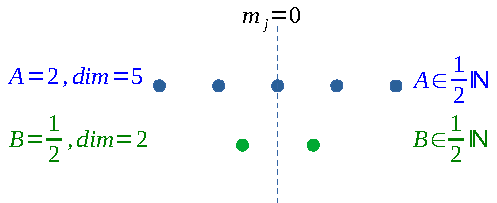
\includegraphics{images/tensor_product.pdf}
    \caption{Two irreps of $\mathfrak{su}(2)_\mathbb{C}\simeq\mathfrak{sl}(2,\mathbb{C})$.}
    \labfig{tensorproduct}
\end{figure}
We take a look at the \textbf{tensor product}\marginnote{The tensor product is essentially the direct sum at the level of the algebra}:
\[
{\color{red}\pi_A\otimes\pi_B=\pi_{A,B}}
\]
{\fontencoding{U}\fontfamily{futs}\selectfont\char 66\relax}
The representation $\pi_A\oplus\pi_B=\pi_{A,B}$ is in general \textbf{not irreducible}. It contains an \textbf{irrep} with the \textbf{highest weight} ("spin") {\color{red}$A+B$}.
\begin{example}1)
\[
\begin{array}{ccccccc}
    \pi_{1/2} & \otimes & \pi_{1/2} & = & \pi_{\underset{\mathclap{\tikz \node {$\uparrow$} node [below=1ex] {\footnotesize Sum $A+B$ of highest weight};}}{1}} & \oplus & \pi_0 \\
\end{array}
\]
Sometimes this is written looking just at the space
\[
\begin{array}{ccccccc}
    \mathbb{C}^2 & \otimes & \mathbb{C}^2 & \cong & \mathbb{C}^3 & \oplus & \mathbb{C}^1 \\ 
    2 & \otimes & 2 & = & 3 & \oplus & 1
\end{array}
\]
2)
\[
\begin{array}{ccccccc}
    \pi_2 & \otimes & \pi_{1/2} & \cong & \pi_{5/2} & \oplus & \pi_{3/2} \\
    \mathbb{C}^5 & \otimes & \mathbb{C}^2 & \cong & \mathbb{C}^6 & \oplus & \mathbb{C}^4 \\ 
    5 & \otimes & 2 & = & 6 & \oplus & 4
\end{array}
\]
\end{example}
{\fontencoding{U}\fontfamily{futs}\selectfont\char 66\relax}
These representation are \underline{\textbf{not unitary!}}\\ $\pazocal{J}_l=A_l+B_l$ is hermitian so that $e^{-i\theta\pazocal{J}_l}$ is unitary. \raisebox{-\mydepth}{{
\includegraphics[height=1.1\baselineskip]{images/smile.jpg}}}\\
$\pazocal{K}_l=-i(A_l-B_l)$ is \textbf{not hermitian}. \raisebox{-\mydepth}{{
\includegraphics[height=1.1\baselineskip]{images/anrgysmile.jpeg}}}\\
For the tensor product $\pi_a\otimes\pi_B\equiv(A,B)$ there are some special names:
\[
\begin{cases}
(0,0) &\text{ scalar fields \qquad\qquad $\mathbb{C}$}\\
\left(0,\frac{1}{2}\right),\left(\frac{1}{2},0\right) &\text{ 2-component spinors \quad\quad $\mathbb{C}^2$}\\
\left(\frac{1}{2},\frac{1}{2}\right)  &\text{ Dirac 4-component spinors \quad $\mathbb{C}^4$}\\
(1,0),(0,1) &\text{ anti-symmetric tensor \quad $F^{\mu\nu}=\pm i\varepsilon^{\mu\nu\rho\sigma}F_{\rho\sigma}$}\marginnote{+1 if $(1,0)$ and $-1$ if $(0,1)$}
\end{cases}
\]
\[
\text{Symmetries} 
\left\{
\begin{aligned}
&\text{space-time: \quad \underline{SR}: $\mathcal{L},\pazocal{P}$ \; \underline{GR}: Diff$(\mathbb{M})$}\\
&\text{internal symmetries: }
\left\{
\begin{aligned}
&\text{U}(1)\\
&\text{SU}(2)\\
&\text{SU}(3)
\end{aligned}
\right.
\end{aligned}
\right.
\]
What is remarkable is that all the groups which appear here (except for ???) are Lie groups. In a sense, the theory we developed covers both kinematic symmetries of our theory and internal symmetries. The professor thinks that it relates to what Freeman Dyson
call the \textit{\href{https://en.wikipedia.org/wiki/The_Unreasonable_Effectiveness_of_Mathematics_in_the_Natural_Sciences}{The Unreasonable Effectiveness of Mathematics in the Natural Sciences}}. Modern science started with a sentence by Galileo:

"\textit{La filosofia è scritta in questo grandissimo libro che continuamente ci sta aperto innanzi a gli occhi (io dico l'universo), ma non si può intendere se prima non s'impara a intender la lingua, e conoscer i caratteri, ne' quali è scritto. Egli è scritto in lingua matematica, e i caratteri son triangoli, cerchi, e altre figure geometriche, senza i quali mezzi è impossibile a intenderne umanamente parola; senza questi è un aggirarsi vanamente per un oscuro laberinto.}"
\begin{marginfigure}
	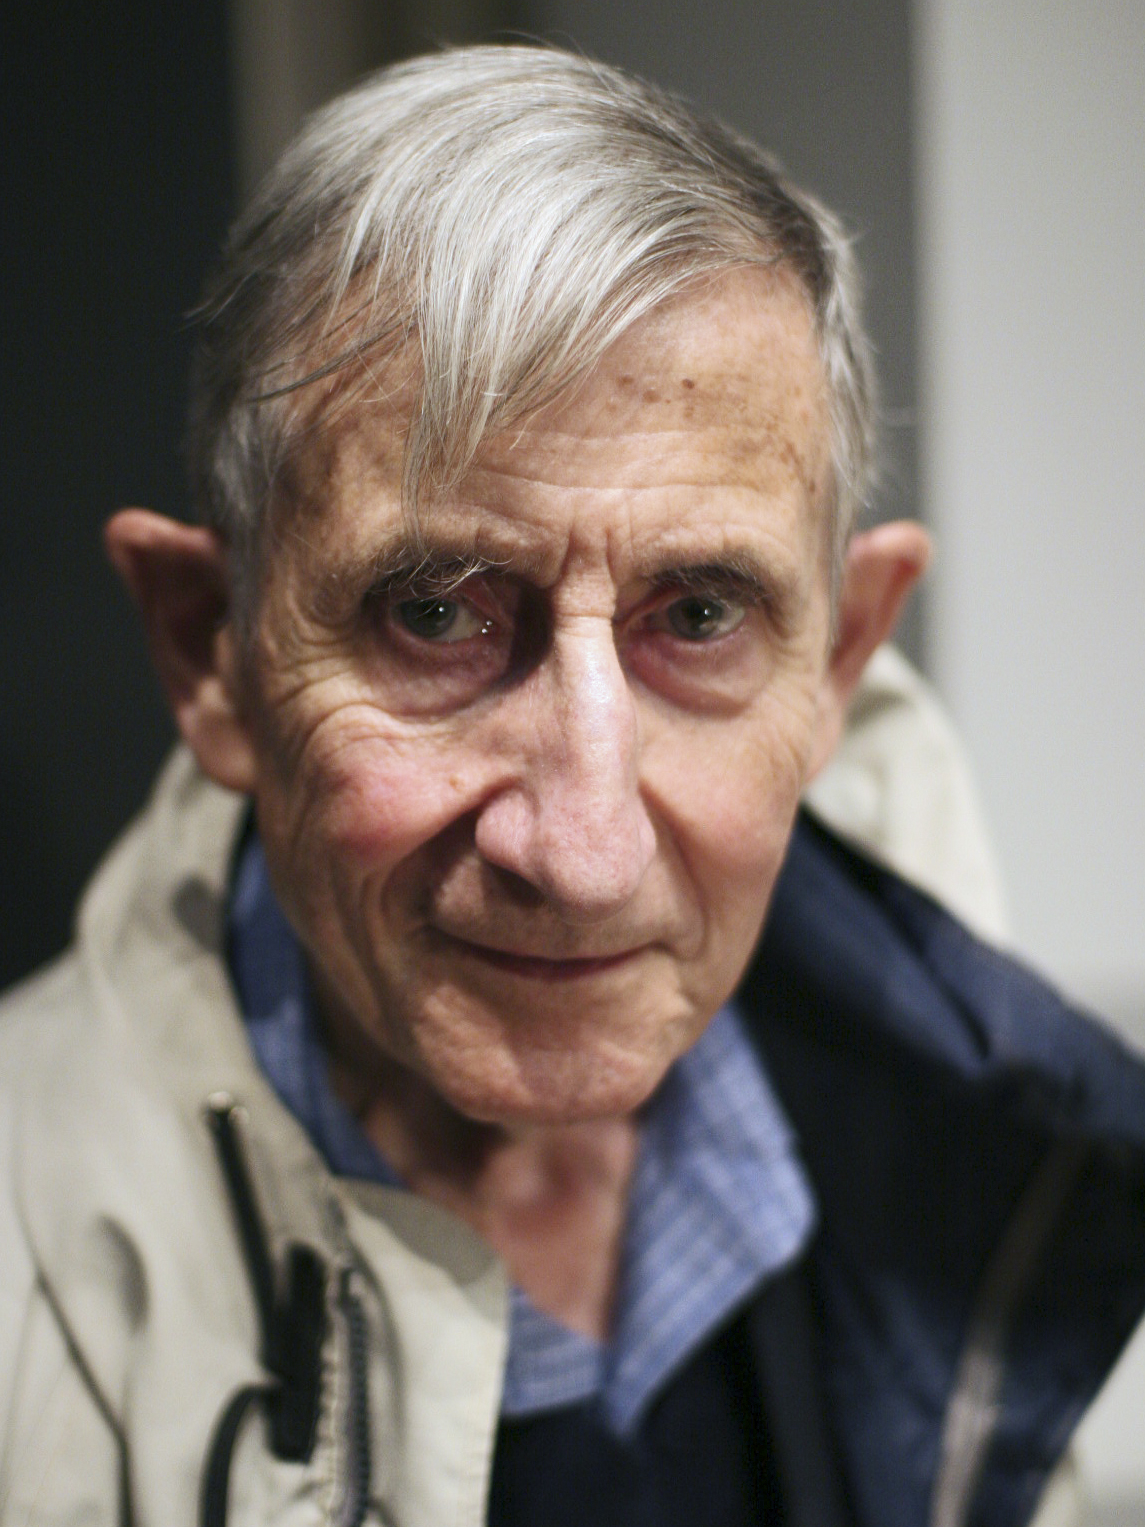
\includegraphics[width=1\linewidth]{images/Freeman_Dyson_(2005).jpeg}
	\caption[Photo of Freeman John Dyson]{From \href{https://commons.wikimedia.org/wiki/File:Freeman_Dyson_(2005).jpg}{Wikimedia:} Freeman John Dyson FRS (15 December 1923 – 28 February 2020) was an English-American theoretical physicist and mathematician known for his works in quantum field theory, astrophysics, random matrices, mathematical formulation of quantum mechanics, condensed matter physics, nuclear physics, and engineering. He was Professor Emeritus in the Institute for Advanced Study in Princeton and a member of the Board of Sponsors of the Bulletin of the Atomic Scientists. Dyson died on 28 February 2020 at a hospital near Princeton, New Jersey, from complications following a fall. He was 96.}
	\labfig{Dyson}
\end{marginfigure}
Which means that the book of nature is written in mathematical fonts. This was extremely successful in the last three/four centuries, but actually we do not know why Mathematics is so effective in our description of the physical world.

\end{document}